\documentclass[spanish]{beamer}
\usepackage[ansinew]{inputenc} % Acepta caracteres en castellano
\usepackage[spanish]{babel}    % silabea palabras castellanas
\usepackage{amsmath}
\usepackage{mathtools,cancel} % cancela con una flecha \cancelto{0}{XXXX}
\renewcommand{\CancelColor}{\color{red}} %change cancel color to red
\usepackage{amsfonts}
\usepackage{amssymb}
\usepackage{dsfont}
\usepackage{graphicx}
\usepackage{geometry}
\usetheme{Madrid}
\usecolortheme{beaver}
\usepackage{textpos}
% Logo  en el comienzo 
\addtobeamertemplate{frametitle}{}{%
\begin{textblock*}{100mm}(.85\textwidth,-1cm)
{\includegraphics[height=0.4in, keepaspectratio=true]{/Users/luisnunez/Dropbox/MisDocumentos/UIS/UISImagenInstitucional/UISLOGO.png}}
\end{textblock*}}

\begin{document}

\title{\textbf{Tres enfoques para un problema} \\
{\bf Part�cula Cargada en un Campo Magn�tico} }
\author[L.A. N��ez]{\textbf{Luis A. N��ez}}  
\institute[UIS]{\textit{Escuela de F�sica, Facultad de Ciencias, } \\
\textit{Universidad Industrial de Santander, Santander, Colombia } \\
{\includegraphics[height=0.4in, keepaspectratio=true]{/Users/luisnunez/Dropbox/MisDocumentos/UIS/UISImagenInstitucional/UISLOGO.png}}
}
\date{\today}
\maketitle


\begin{frame}
\frametitle{Agenda}
  \tableofcontents
\end{frame}


%%%%% Diapo 1
\section{El problema}
\frame{
\frametitle{El problema y el enfoque Lagrangeano}
   \begin{itemize}  
  	\item<1-> {\bf Sistema f�sico}
	\begin{itemize}
  	\item Masa \( m \), carga \( q \), movimiento en plano \( xy \)
  	\item Campo magn�tico uniforme: \( \mathbf{B} = B \hat{z} \), sin campo el�ctrico: \( \mathbf{E} = 0 \)
  	\item Potencial vectorial $\mathbf{B} = \nabla \times \mathbf{A}$ en el calibre de Landau tenemos $\mathbf{A} = (0, Bx, 0)$ y adem�s $\mathbf{A} \cdot \dot{\mathbf{r}} = Bx \dot{y}$
	\end{itemize}
	\item<2-> {\bf El lagrangiano del sistema} \\
	$\mathcal{L} = \frac{1}{2} m (\dot{x}^2 + \dot{y}^2) + q \mathbf{A}\cdot \dot{\mathbf{r}} \equiv \mathcal{L}(x, y, \dot{x}, \dot{y}) = \frac{1}{2} m (\dot{x}^2 + \dot{y}^2) + q B x \dot{y}$
	\item<3-> {\bf Ecuaciones de Euler-Lagrange}
	\begin{itemize}
	\item Para \( x \): $\frac{d}{dt}(m \dot{x}) - q B \dot{y} = 0 \Rightarrow m \ddot{x} = q B \dot{y}$
	\item Para \( y \): $\frac{d}{dt}(m \dot{y} + q B x) = 0 \Rightarrow m \ddot{y} = -q B \dot{x}$
	\item Sistema resultante: $\ddot{x} = \omega_c \dot{y}, \quad \ddot{y} = -\omega_c \dot{x}$  Dos ecuaciones acopladas, donde $\omega_c = \frac{q B}{m}$ es frecuencia de ciclotr�n
	\item Derivando: $\dddot{x} = \omega_c \ddot{y} = -\omega_c^2 \dot{x} \Rightarrow \ddot{x} + \omega_c^2 x = 0$, tambi�n $\ddot{y} + \omega_c^2 y = 0$
	\item Ecuaciones de oscilador arm�nico para \( x(t) \) y \( y(t) \) con soluci�n
	\item $x(t) = A \cos(\omega_c t) + B \sin(\omega_c t)$ y  $y(t) = C \cos(\omega_c t) + D \sin(\omega_c t)$
	\item La part�cula describe una �rbita circular con \( |\mathbf{v}| = \text{cte} \) y $R = \frac{v_0}{\omega_c}$
	\end{itemize}
\end{itemize}
}
%%%%% Diapo 2
\section{Formalismo Hamiltoniano}
\frame{
\frametitle{Formalismo Hamiltoniano}
\begin{itemize}  
	\item<1-> El hamiltoniano se define por: $\mathcal{H} = p_x \dot{x} + p_y \dot{y} - \mathcal{L}$
	\item<2-> Con $p_x = \frac{\partial \mathcal{L}}{\partial \dot{x}} = m \dot{x} \quad$ y $\quad p_y = \frac{\partial \mathcal{L}}{\partial \dot{y}} = m \dot{y} + q B x$
	\item<3-> Entonces $\mathcal{H} = \frac{p_x^2}{2m} + \frac{1}{2m} (p_y - q B x)^2$
	\item<4-> Las Ecuaciones de Hamilton $\dot{x} = \frac{\partial H}{\partial p_x} = \frac{p_x}{m}
\quad \Rightarrow \quad \ddot{x} = \frac{\dot{p}_x}{m}$ $\dot{p}_x = -\frac{\partial H}{\partial x} = -\frac{q B}{m} (p_y - q B x); \quad$ $\dot{y} = \frac{\partial H}{\partial p_y} = \frac{p_y - q B x}{m}
\quad \Rightarrow \ddot{y} = \frac{\dot{p}_y - q B \dot{x}}{m}$; finalmente $\dot{p}_y = -\frac{\partial H}{\partial y} = 0 \quad \Rightarrow \quad p_y = \text{cte}$

\end{itemize}
}
%
%%%%% Diapo 2
\section{Secci�n}
\frame{
\frametitle{T�tulo transparencia}
\begin{itemize}  
	\item<1-> 
\end{itemize}
}


%%%%% Diapo Fin
\section{Recapitulando}
\frame{
  \frametitle{Recapitulando}
En presentaci�n consideramos
  \begin{enumerate}
  	\item<1->
   \end{enumerate}
}

  
\end{document}
%%%%% Diapo 2
\section{Secci�n}
\frame{
\frametitle{T�tulo transparencia}
\begin{itemize}  
	\item<1-> 
\end{itemize}
}

	\begin{figure}[t]
		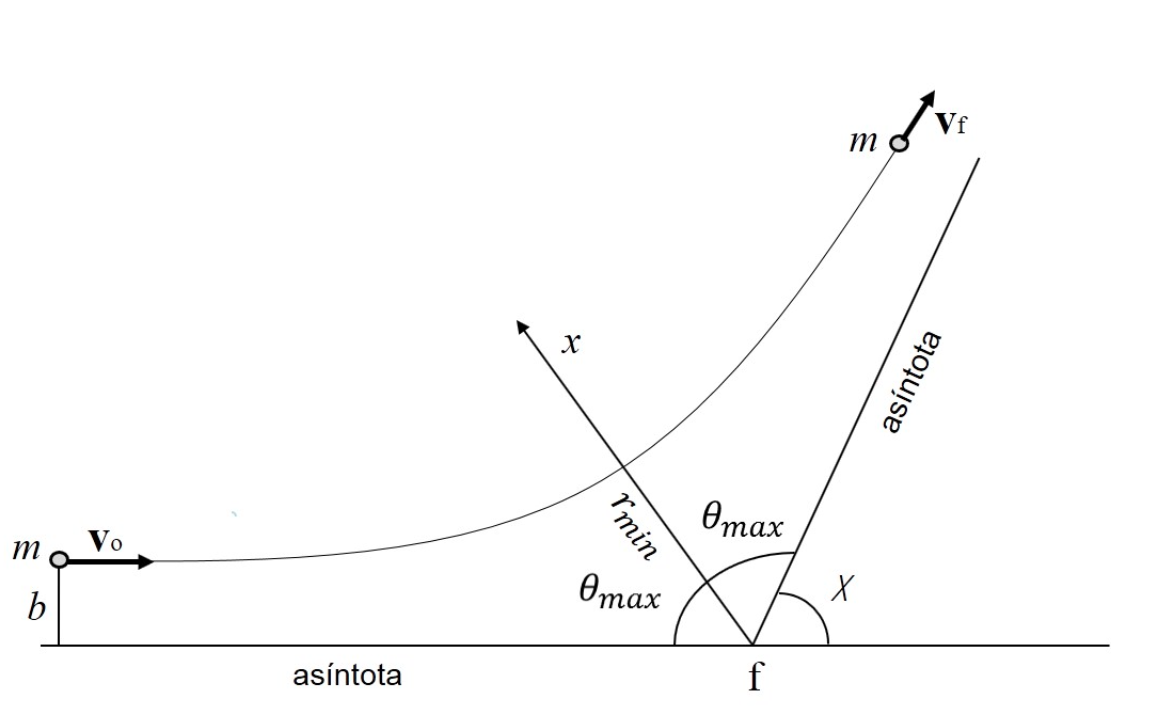
\includegraphics[width=1.8in]{Figuras/Dispersion.png}
   	\end{figure}
	
